\chapter{Result and Discussion} \label{Discussion}

In this chapter, we will discuss our results and evaluate the performance of the machine learning approach compared to the traditional method. Our network performs a outstanding reconstruct efficiency on both event level and quark level reconstruction. 

\section{Invariant mass and reconstruct efficiency }\label{sec:inv mass and reco eff}

Before discussing the result, we should define the category for the reconstruction efficiency. Treating the truth matching result as the target, the prediction of $\chi^{2}$ or SPA-NET may produce three kinds of results:

\begin{itemize}
	\item Correct matched: An event in which both top quarks are correctly predicted by the reconstruction method.
	\item Incorrect matched: An event that one or both top quarks is incorrectly predicted by the reconstruction method.
	\item Unmatched: An event that one of the truth match results contains an element that does not match to any jets.
\end{itemize}
Based on the category above, the reconstruction efficiency can be computed. The reconstruction efficiency is separated into two components: event-based efficiency and quark-based efficiency. The event-based efficiency is calculated based on how many \textbf{events} are matched correctly, incorrectly, and unmatched. The quark-based efficiency is based on how much \textbf{top quarks} are assigned correctly. The efficiency is shown in the table below:
\\
\begin{table}[H]
	%\captionsetup{justification=raggedright,singlelinecheck=false}
	\caption{Using $\epsilon$ as the symbol of efficiency. This table performs the efficiencies of the $\chi^2$ and SPA-NET assignments assessed by per-event efficiency $\epsilon^{\rm event}$ and per-top efficiencies $\epsilon^{\rm top}$ inclusively and by jet multiplicity \Njets. The subscript of $\epsilon^{\rm top}_{1}$ and $\epsilon^{\rm top}_{2}$ is stands for the one/two reconstructable events.}
	\centering
	\begin{tabular}{c c  c  c  c c  c}
		\hline
		\hline
		& \multicolumn{3}{c}{$\chi^2$ Method} & \multicolumn{3}{c}{SPA-NET }\\
		\hspace{0.2cm}\Njets & \hspace{0.15cm} \epsevent & $\epstoptwo$ & \hspace{0.15cm} $\epstopone$ \hspace{0.15cm} & \hspace{0.15cm} \epsevent & $\epstoptwo$ & \hspace{0.15cm} $\epstopone$ \hspace{0.15cm}   \\
		\midrule
		6          & 61.8\% & 65.0\% & 24.2\% & 80.7\% & 84.1\% & 56.7\% \\
		7          & 40.8\% & 50.4\% & 24.6\% & 66.8\% & 75.7\% & 56.2\% \\
		$\geq$8    & 23.2\% & 35.5\% & 20.2\% & 52.3\% & 66.2\% & 52.9\% \\
		\midrule     
		\vspace{0.2cm}
		\textbf{Inclusive}  &\textbf{ 37.7}\% & \textbf{47.0}\% & \textbf{23.0\%} & \textbf{63.7}\% &\textbf{73.5}\% &\textbf{55.2\%} \\
		\hline
	\end{tabular}
	\label{tab:eps}
\end{table}
On overall events, the $\chi^{2}$ has performed a $37.7\%$ efficiency, while SPA-NET archieves an efficiency $63.7\%$. The $\chi^{2}$ method had the best performance on the 6 jets category but perform worse where an event contains more than 8 jets. The SPA-NET performs much better than the $\chi^{2}$ in all categories. For the event with two identifiable top quarks, the $\chi^{2}$ method achieved an efficiency $\epsilon^{\rm top}_{2}$ $65.0\%$, but SPA-NET archives an $\epsilon^{\rm top}_{2}$ $84.1\%$. Since we train the SPA-NET with the events that contain two identifiable top quarks, it is reasonable that the $\epsilon^{\rm top}_{1}$ of SPA-NET is lower than $\epsilon^{\rm top}_{2}$. Moreover, since our definition of equation (\ref{eqn:chi2}) is based on the difference between reconstructing invariant masses of two quark candidates, it may be difficult for the $\chi^{2}$ method to assign the jet properly in an event that only contains one identifiable top quark. Note that in our evaluation dataset, 8.1\% of events in which both tops are identifiable have at least one $b$-quark matched to non-$b$-tagged jets, which are impossible for the $\chi^{2}$ method to reconstruct correctly.  These quarks were reconstructed by SPA-NET with an efficiency of 29.4\%.

\subsection{Reconstructed invariant mass }\label{subsec:reco inv mass }

Using $\chi^{2}$ minimization, we may obtain the best assignment under the constraint of parameters. In this project, the parameters are configured as: $m_{\rm W}=81.3$ GeV, $\sigma_{\rm W} = 12.3$ GeV, and $\sigma_{\rm m_{bjj}}=26.3$ GeV. The parameters $\sigma_{\rm W}$ and $\sigma_{\rm m_{bjj}}$ are found by fitting the mass distribution of the W boson and top quark. While computing $\chi^{2}$ value, we use the b-tagging information to assign the b quark candidates. 
\\
The following plots is the reconstructed mass distribution of W boson and top quark using $\chi^{2}$ minimization method and SPA-NET.
\\
\begin{figure}[H]
	\centering
	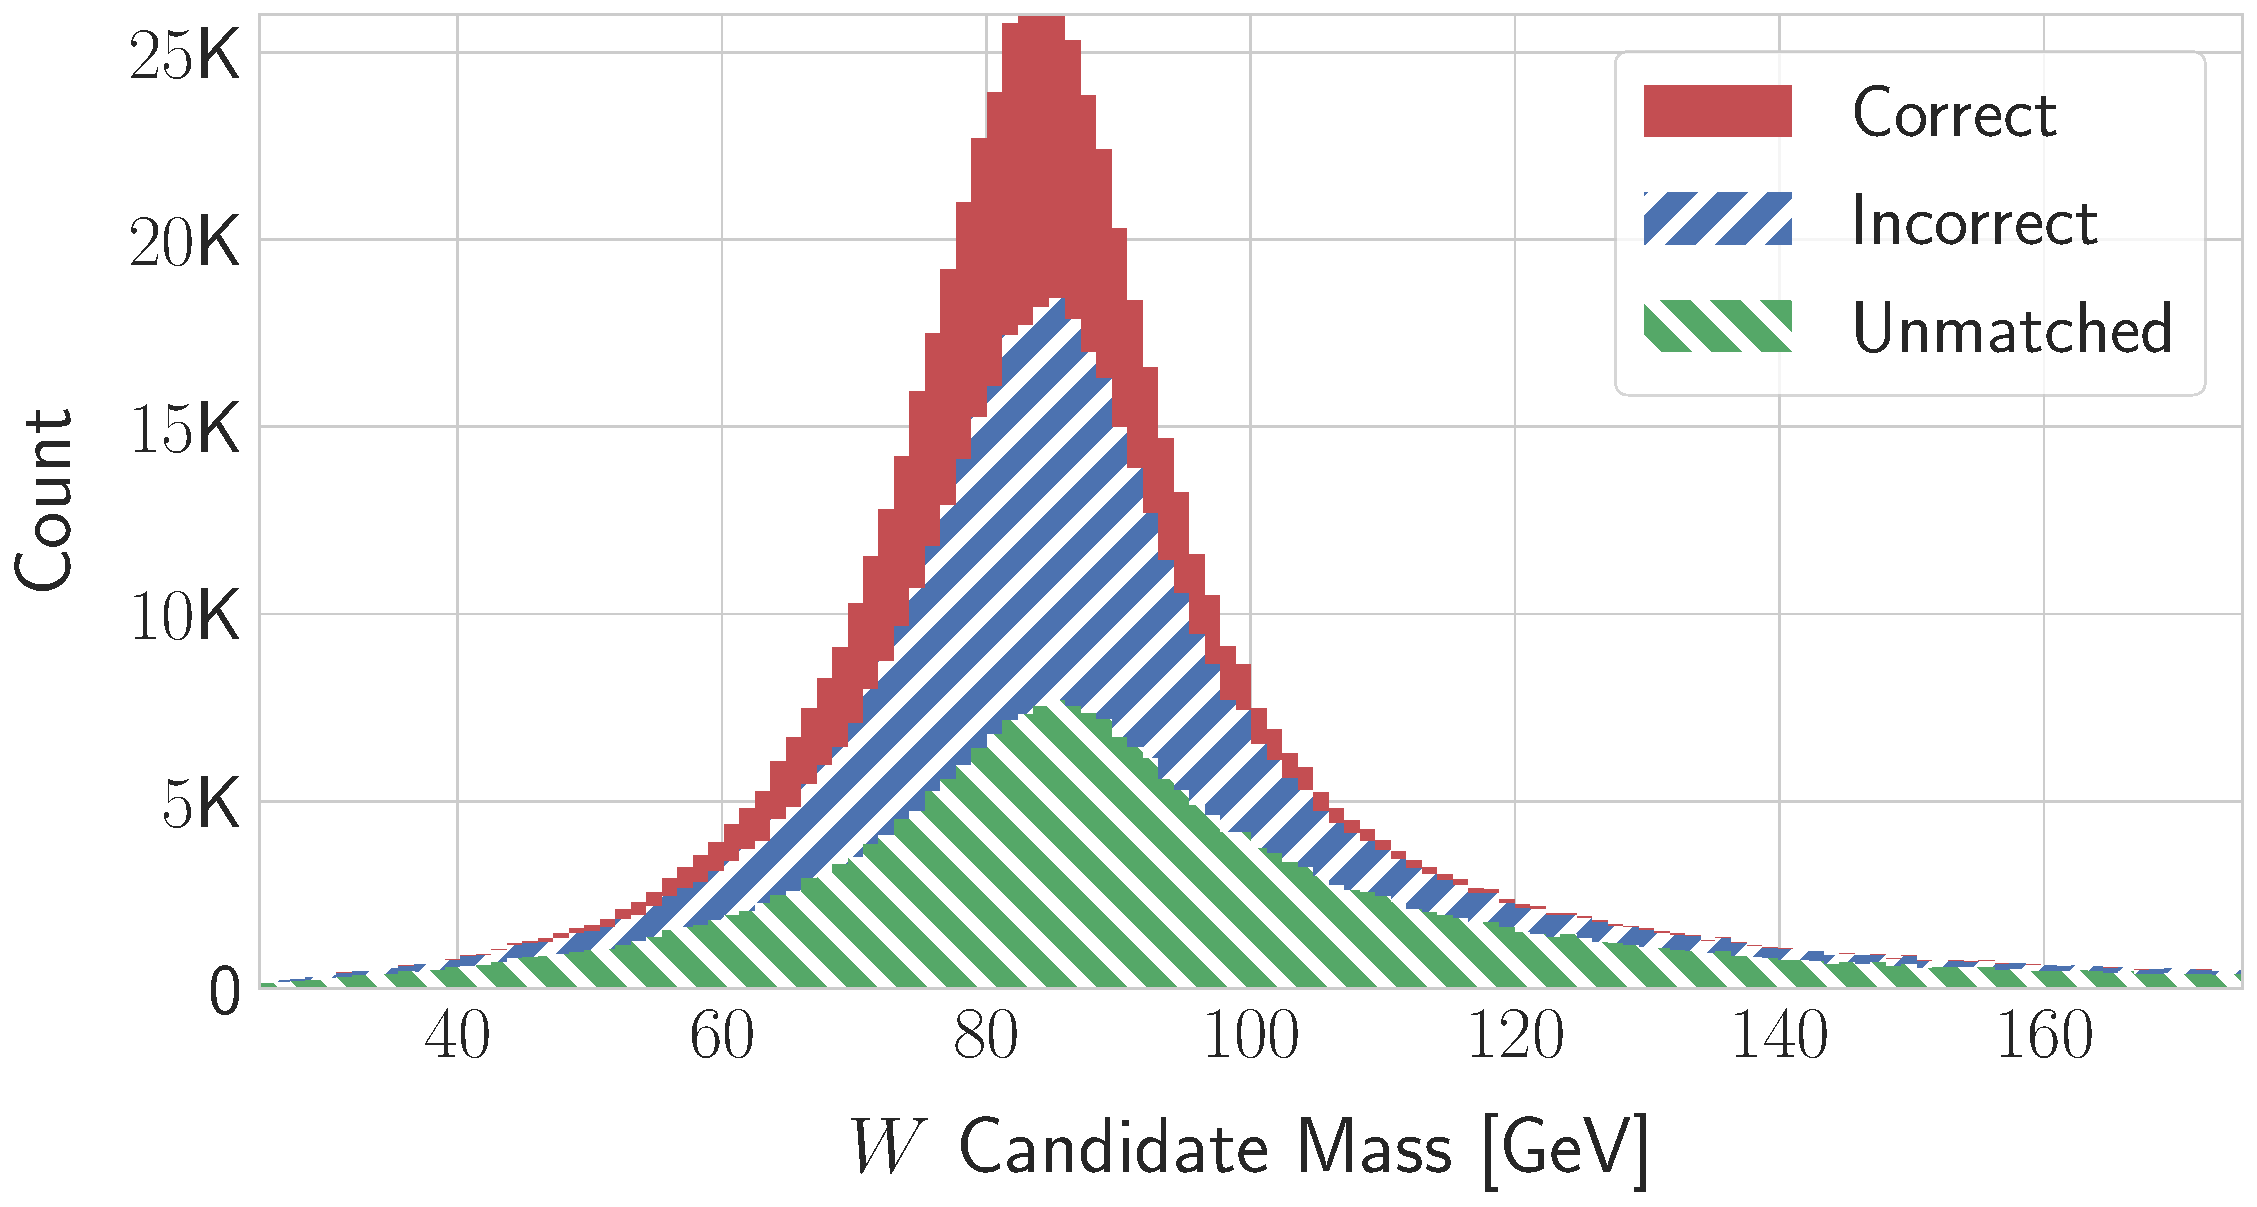
\includegraphics[width=0.7\textwidth]{Figures/network_w_quark_stacked_chi2.pdf}
	\caption{W boson mass reconstructed by $\chi^{2}$ minimization method.}
	\label{fig: chi2 reco Wboson}
\end{figure}
\begin{figure}[H]
	\centering
	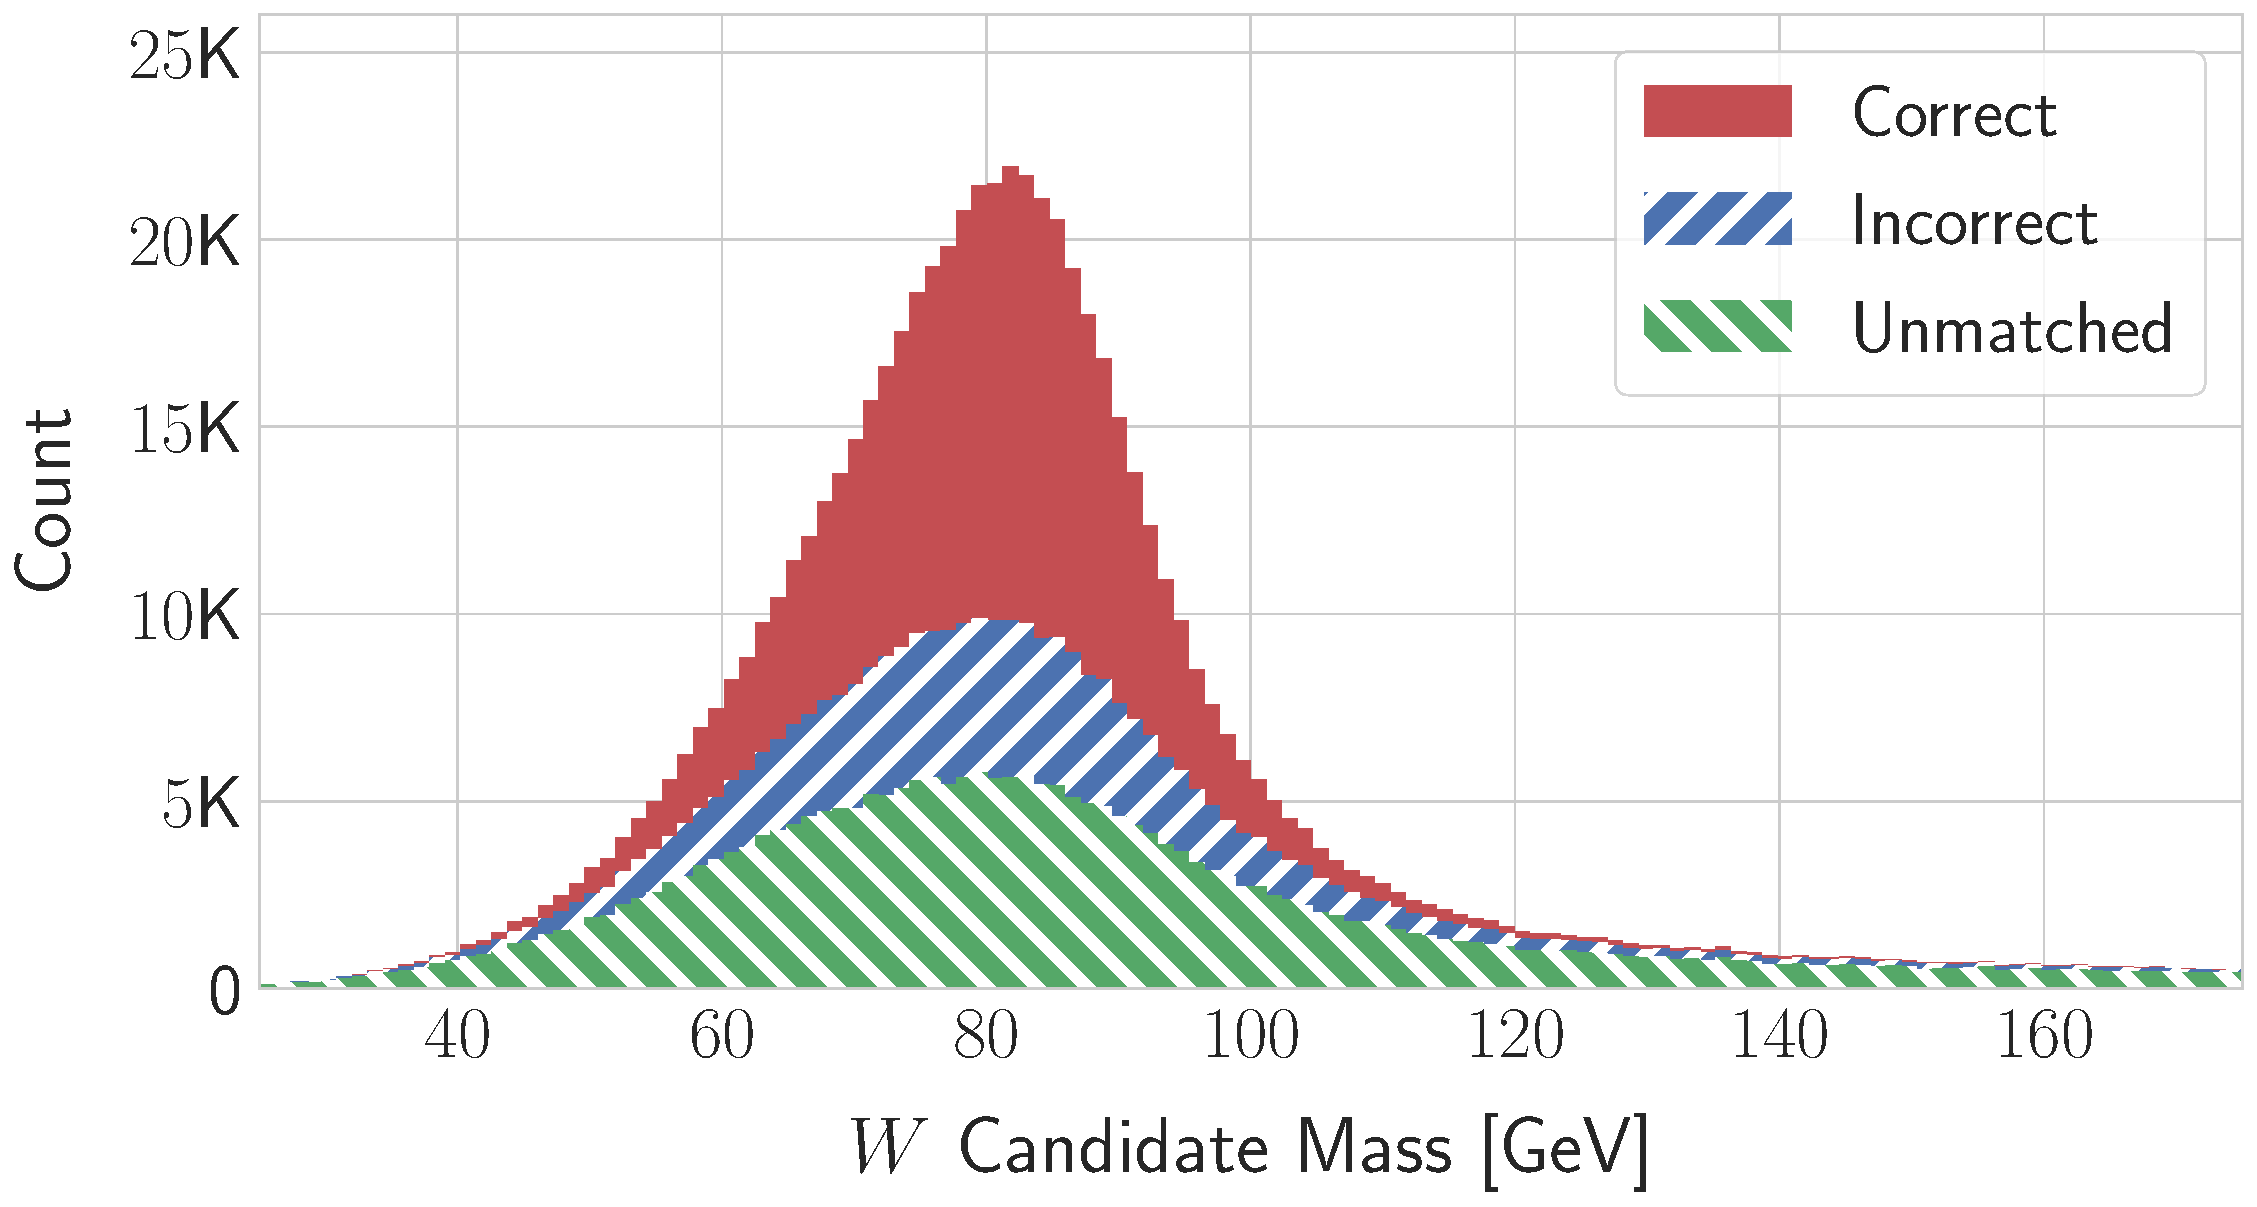
\includegraphics[width=0.7\textwidth]{Figures/network_w_quark_stacked.pdf}
	\caption{W boson mass reconstructed by SPA-NET.}
	\label{fig: spanet reco Wboson}
\end{figure}

\begin{figure}[H]
	\centering
	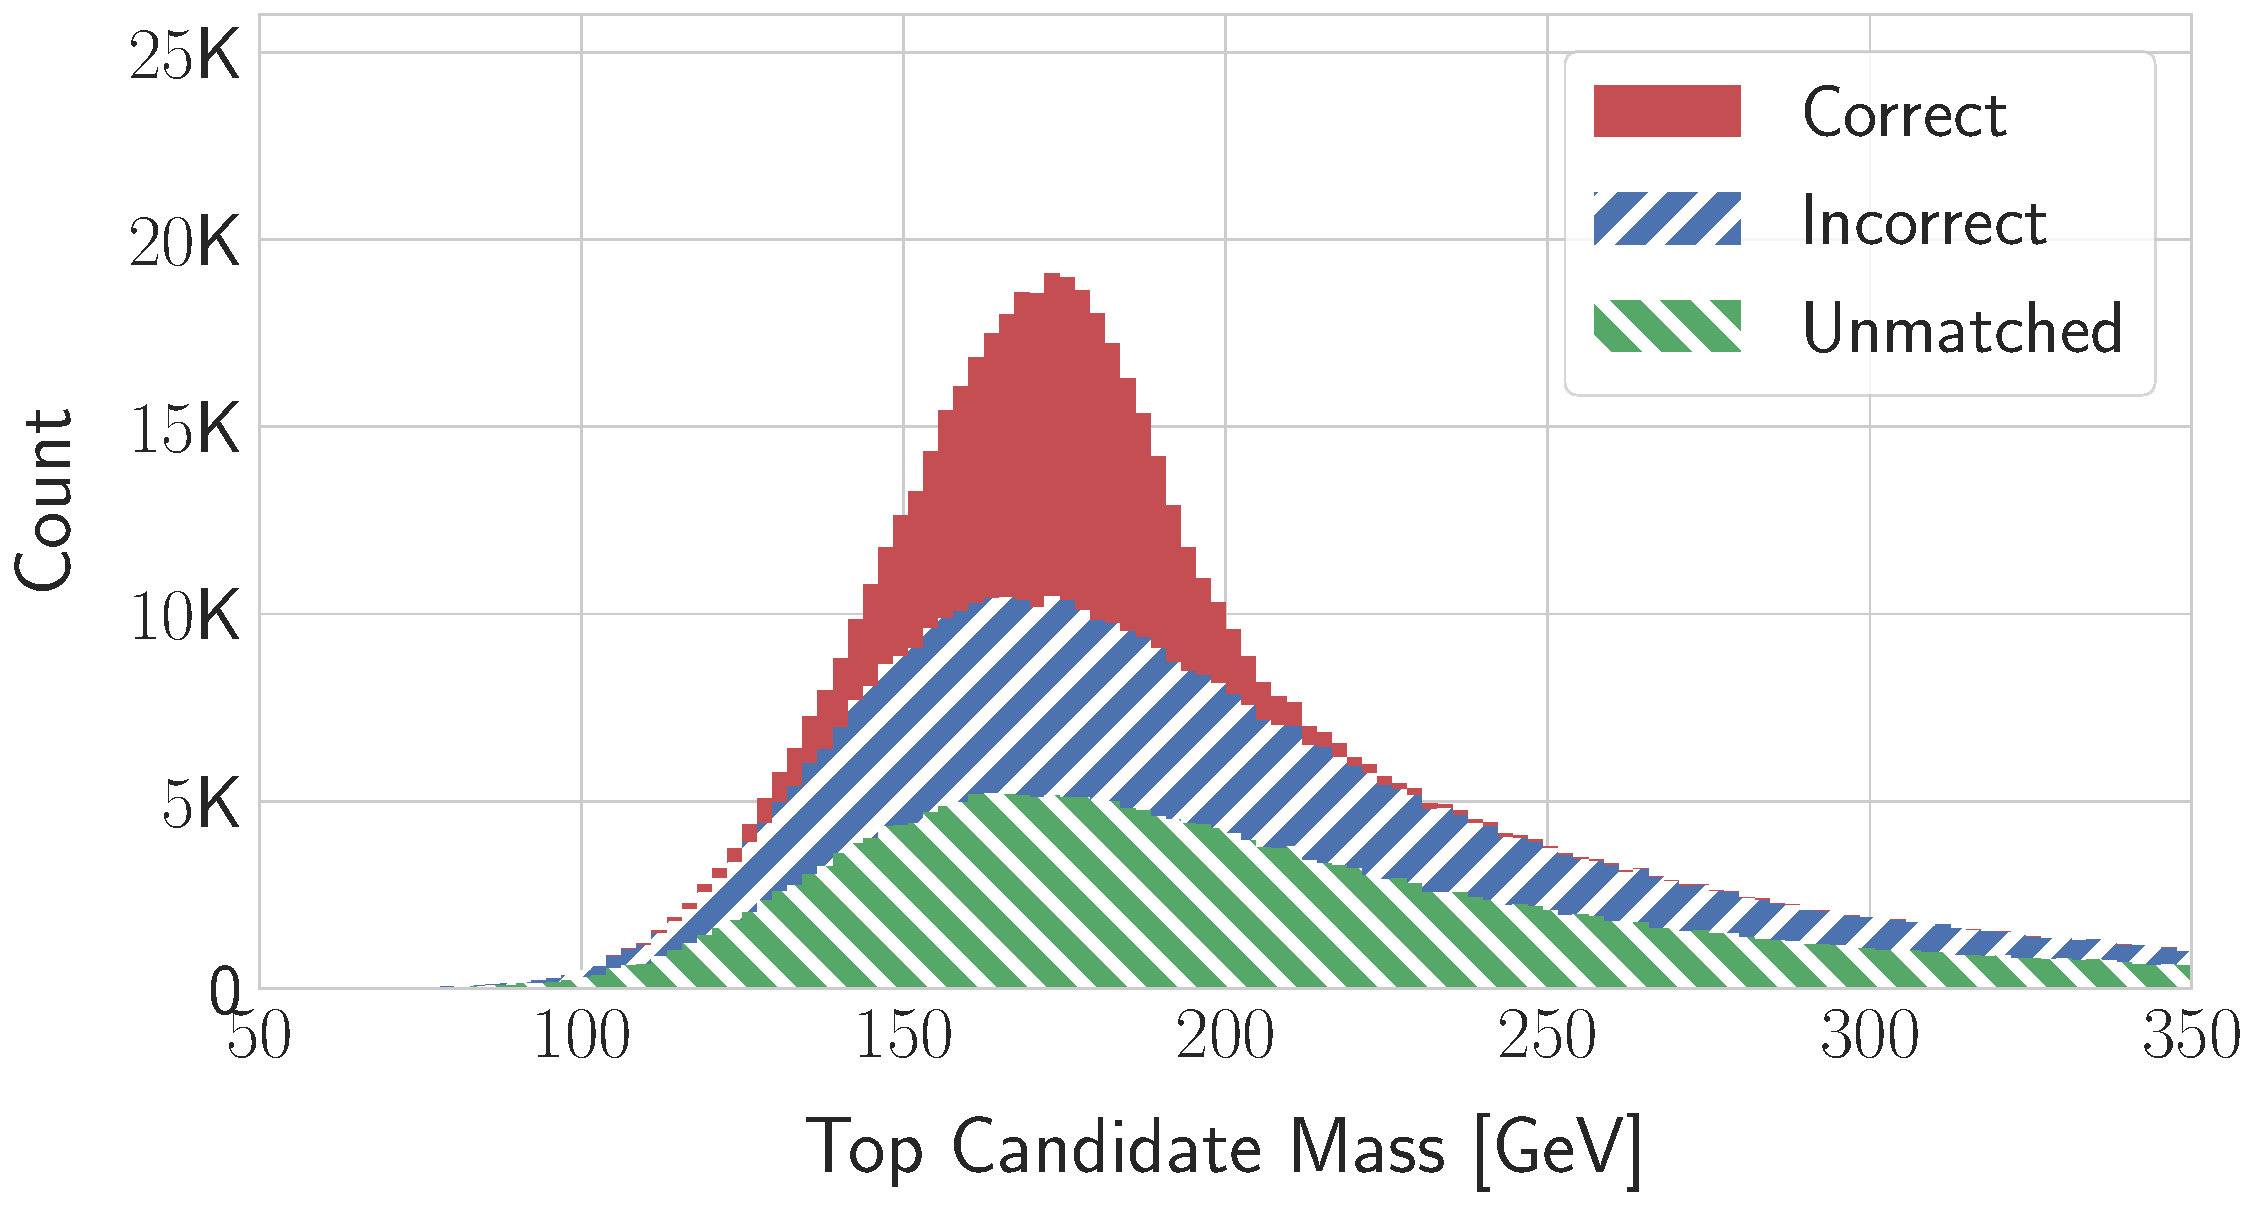
\includegraphics[width=0.7\textwidth]{Figures/network_t_quark_stacked_chi2.pdf}
	\caption{ Top quark mass reconstructed by $\chi^{2}$ minimization method.}
	\label{fig: chi2 reco t quark}
\end{figure}
\begin{figure}[H]
	\centering
	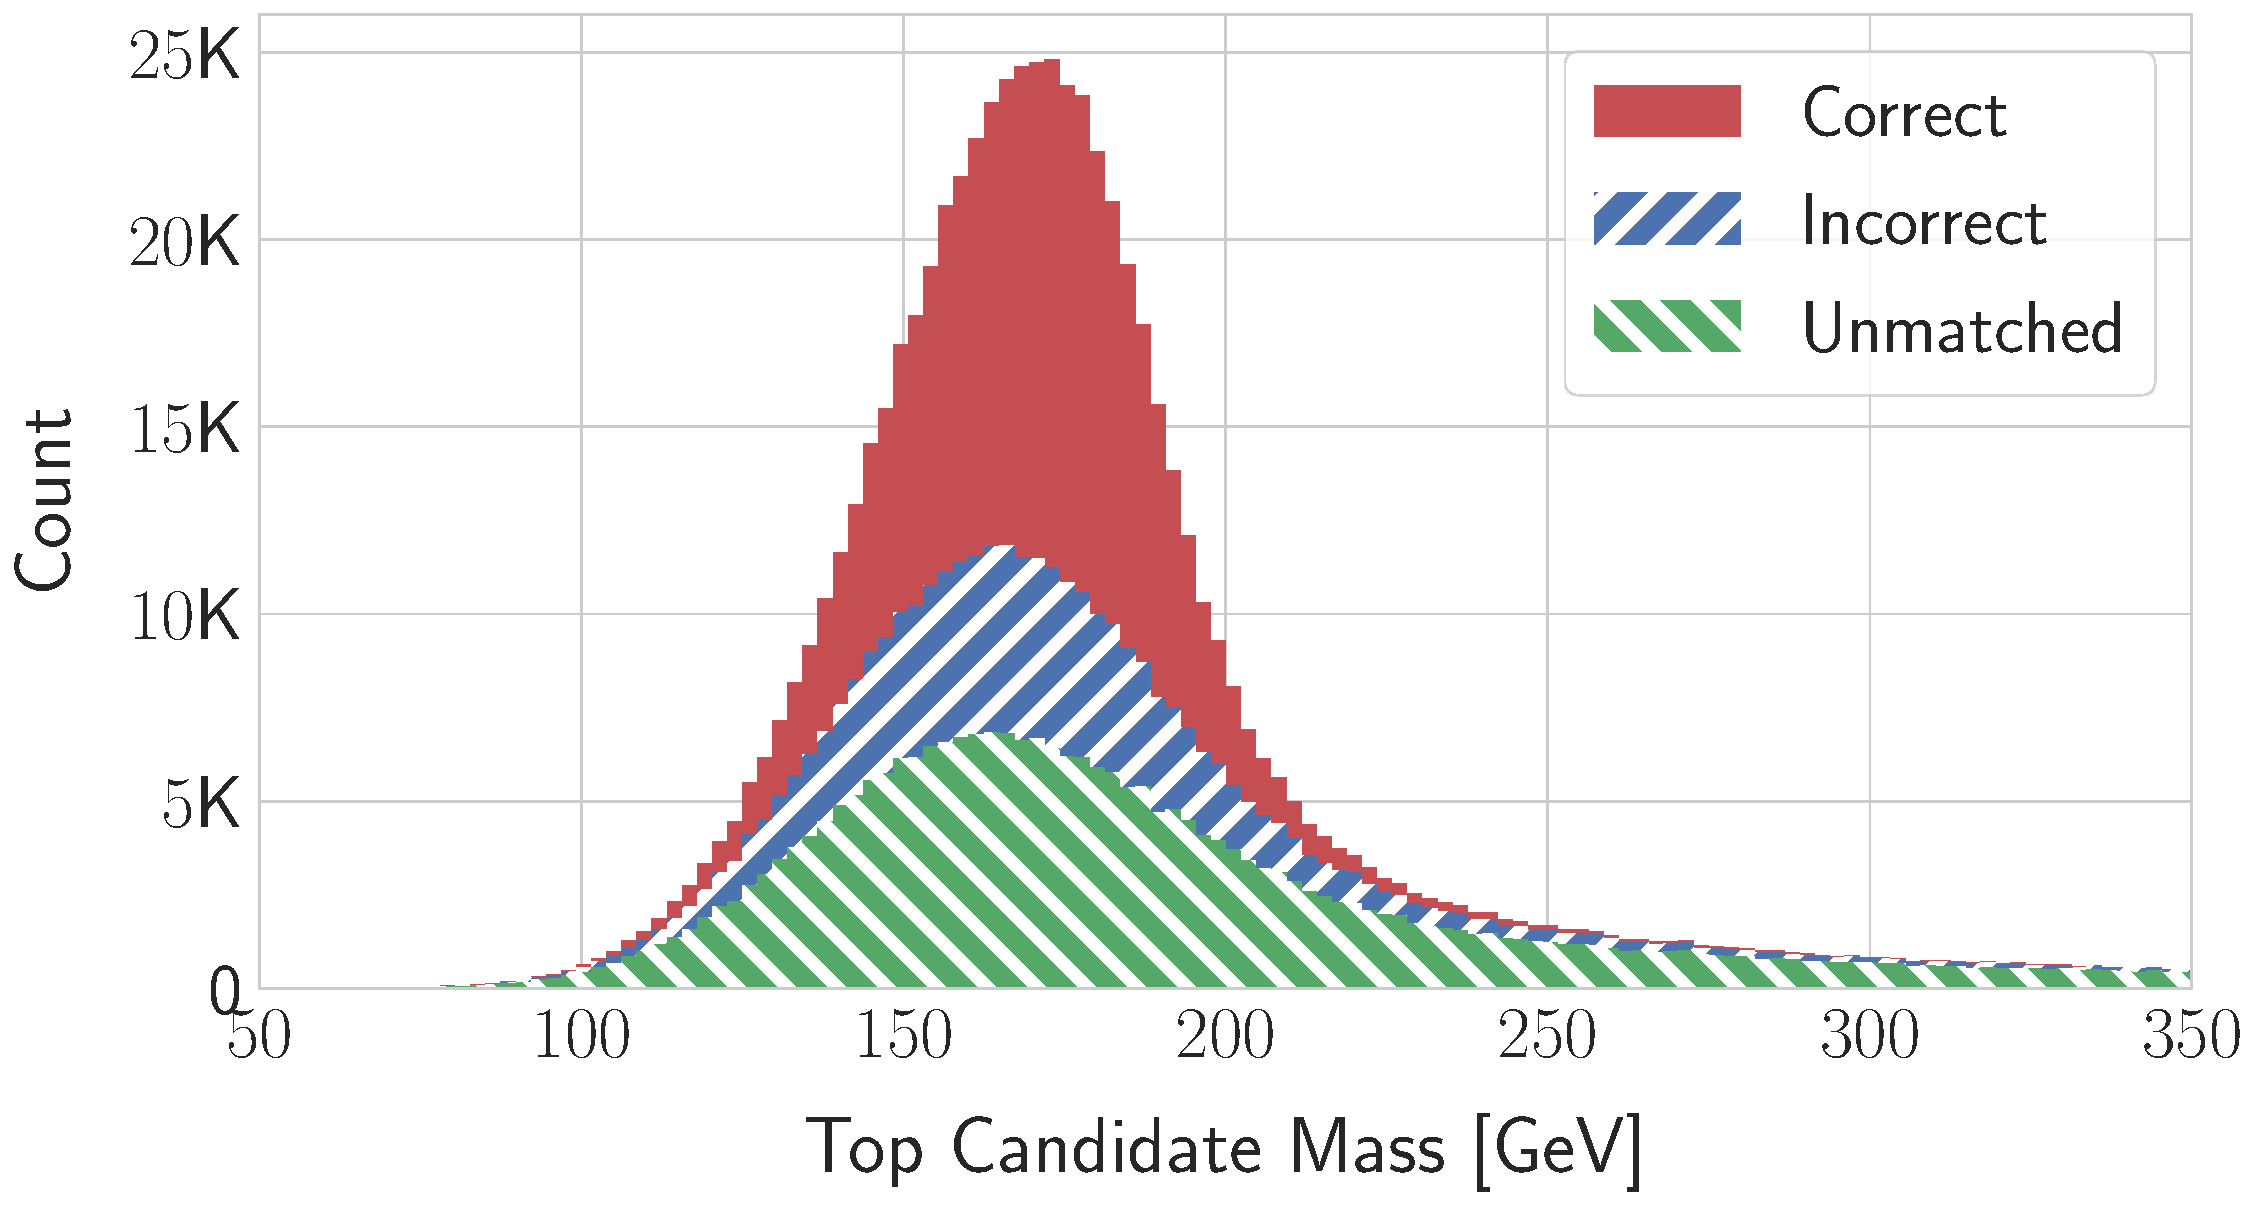
\includegraphics[width=0.7\textwidth]{Figures/network_t_quark_stacked.pdf}
	\caption{ Top quark mass reconstructed by SPA-NET.}
	\label{fig: spanet reco t quark}
\end{figure}
Comparing the result shown in Figure \ref{fig: chi2 reco Wboson} and Figure \ref{fig: spanet reco Wboson}, we found the $\chi^{2}$ method has a narrower peak around W boson mass than the SPA-NET. This narrower peak is due to the incorrect and unmatched events and can be explained by the presence of $m_{\rm W}$ in equation (\ref{eqn:chi2}). Figure \ref{fig: spanet reco t quark} and Figure \ref{fig: chi2 reco t quark} show that the SPA-NET has the more peaked distribution compared to the $\chi^{2}$ method with comparable incorrect/unmatched events.

\subsection{ROC curve}\label{sebsec:roc}
The Receiver operating characteristic (ROC) curve is a useful tool to evaluate the performance of a machine learning model. The ROC curve of SPA-NET applied on events with one and two reconstructable top quarks is shown in Figure \ref{fig: roc one top} and Figure \ref{fig: roc two top}. Note that the targets are defined as 1 if the prediction is correct; 0 if the prediction is incorrect.
\\
 \begin{figure}[H]
 	\centering
 	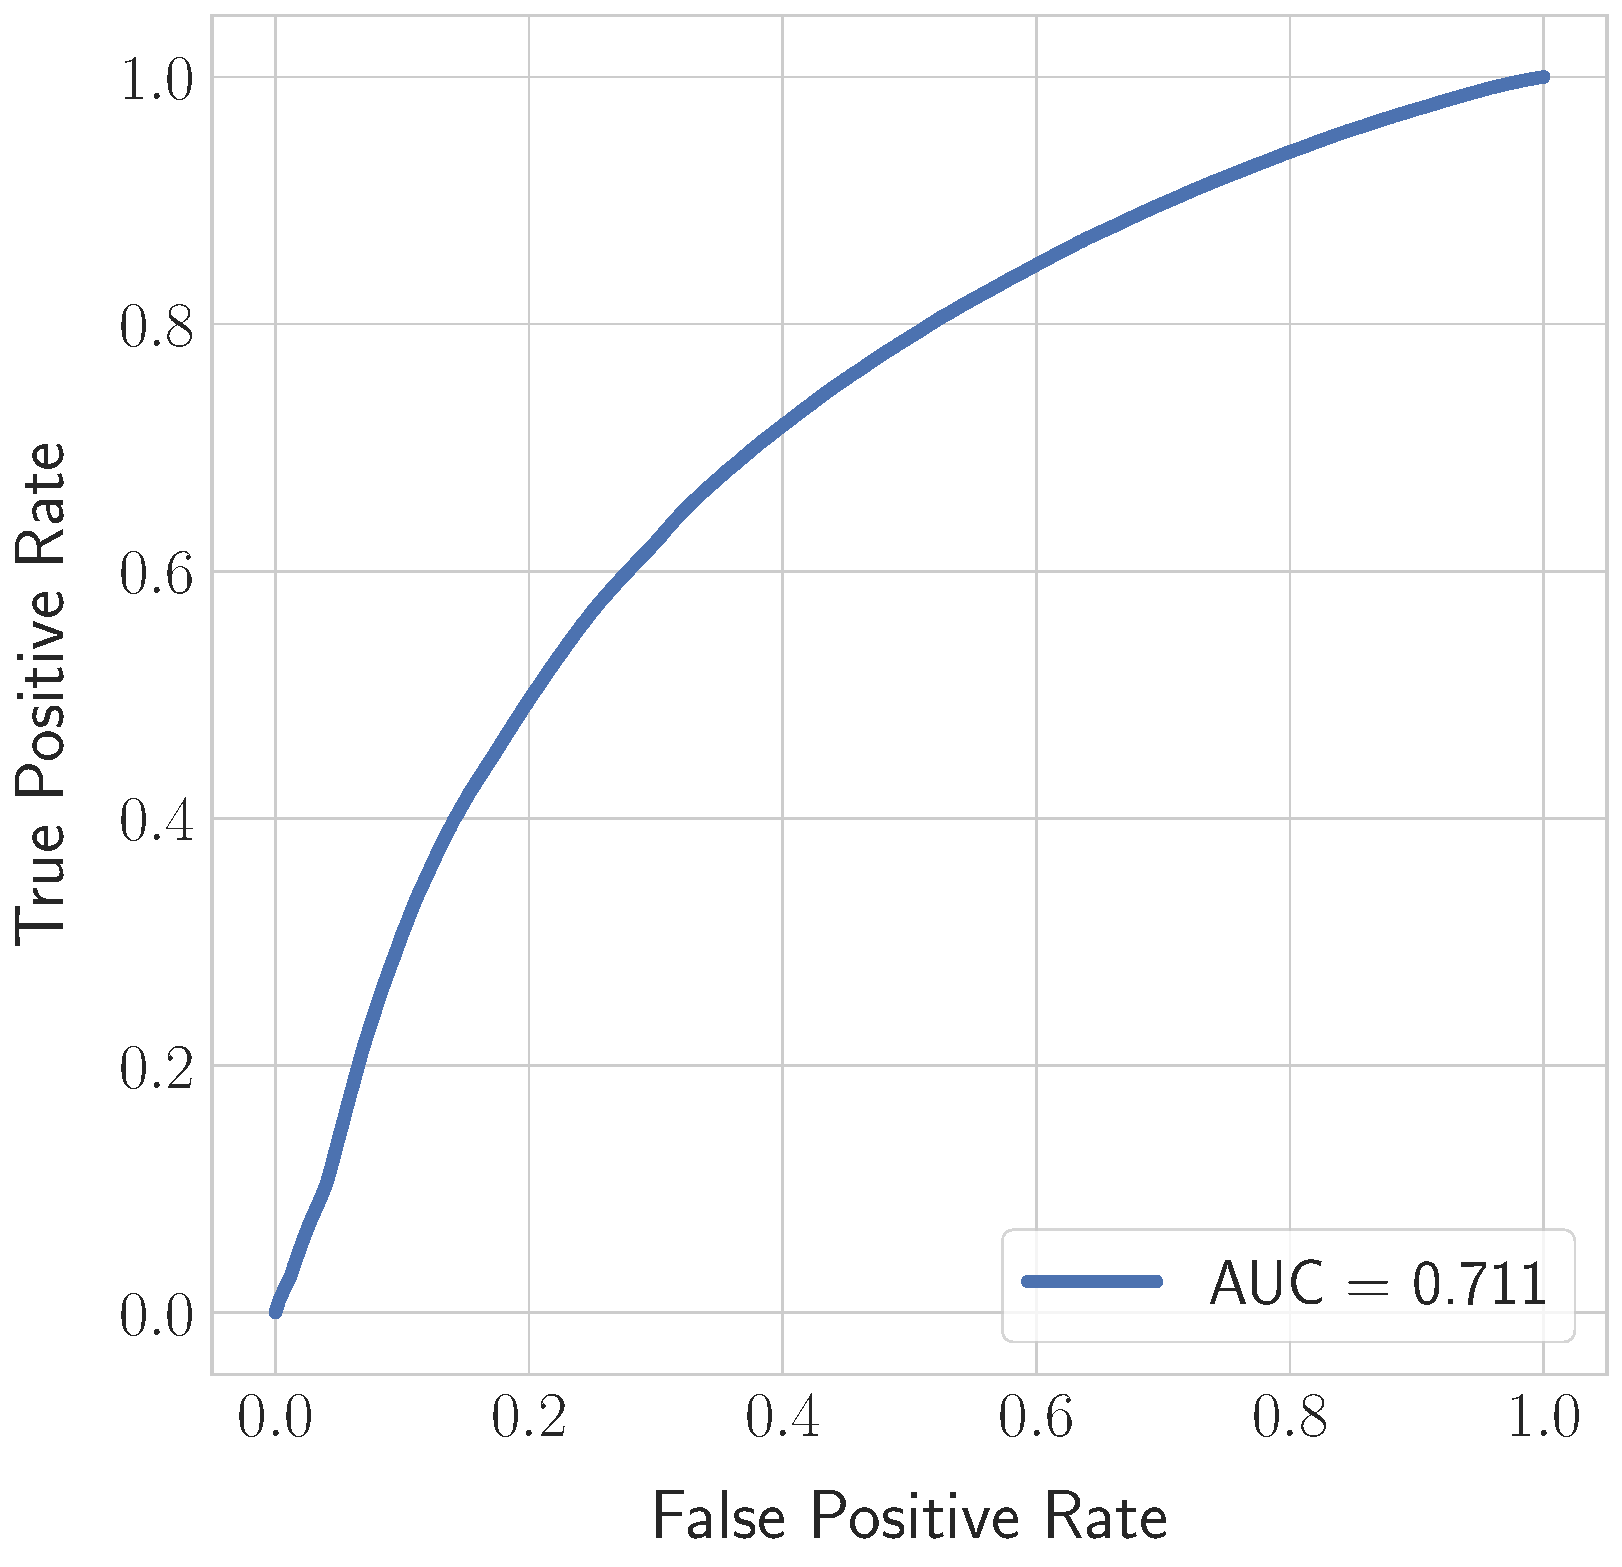
\includegraphics[width=0.6\textwidth]{Figures/roc_one_quark.pdf}
 	\caption{ ROC curve of SPA-NET applies on events with one reconstructable top.}
 	\label{fig: roc one top}
 \end{figure}
 \begin{figure}[H]
 	\centering
 	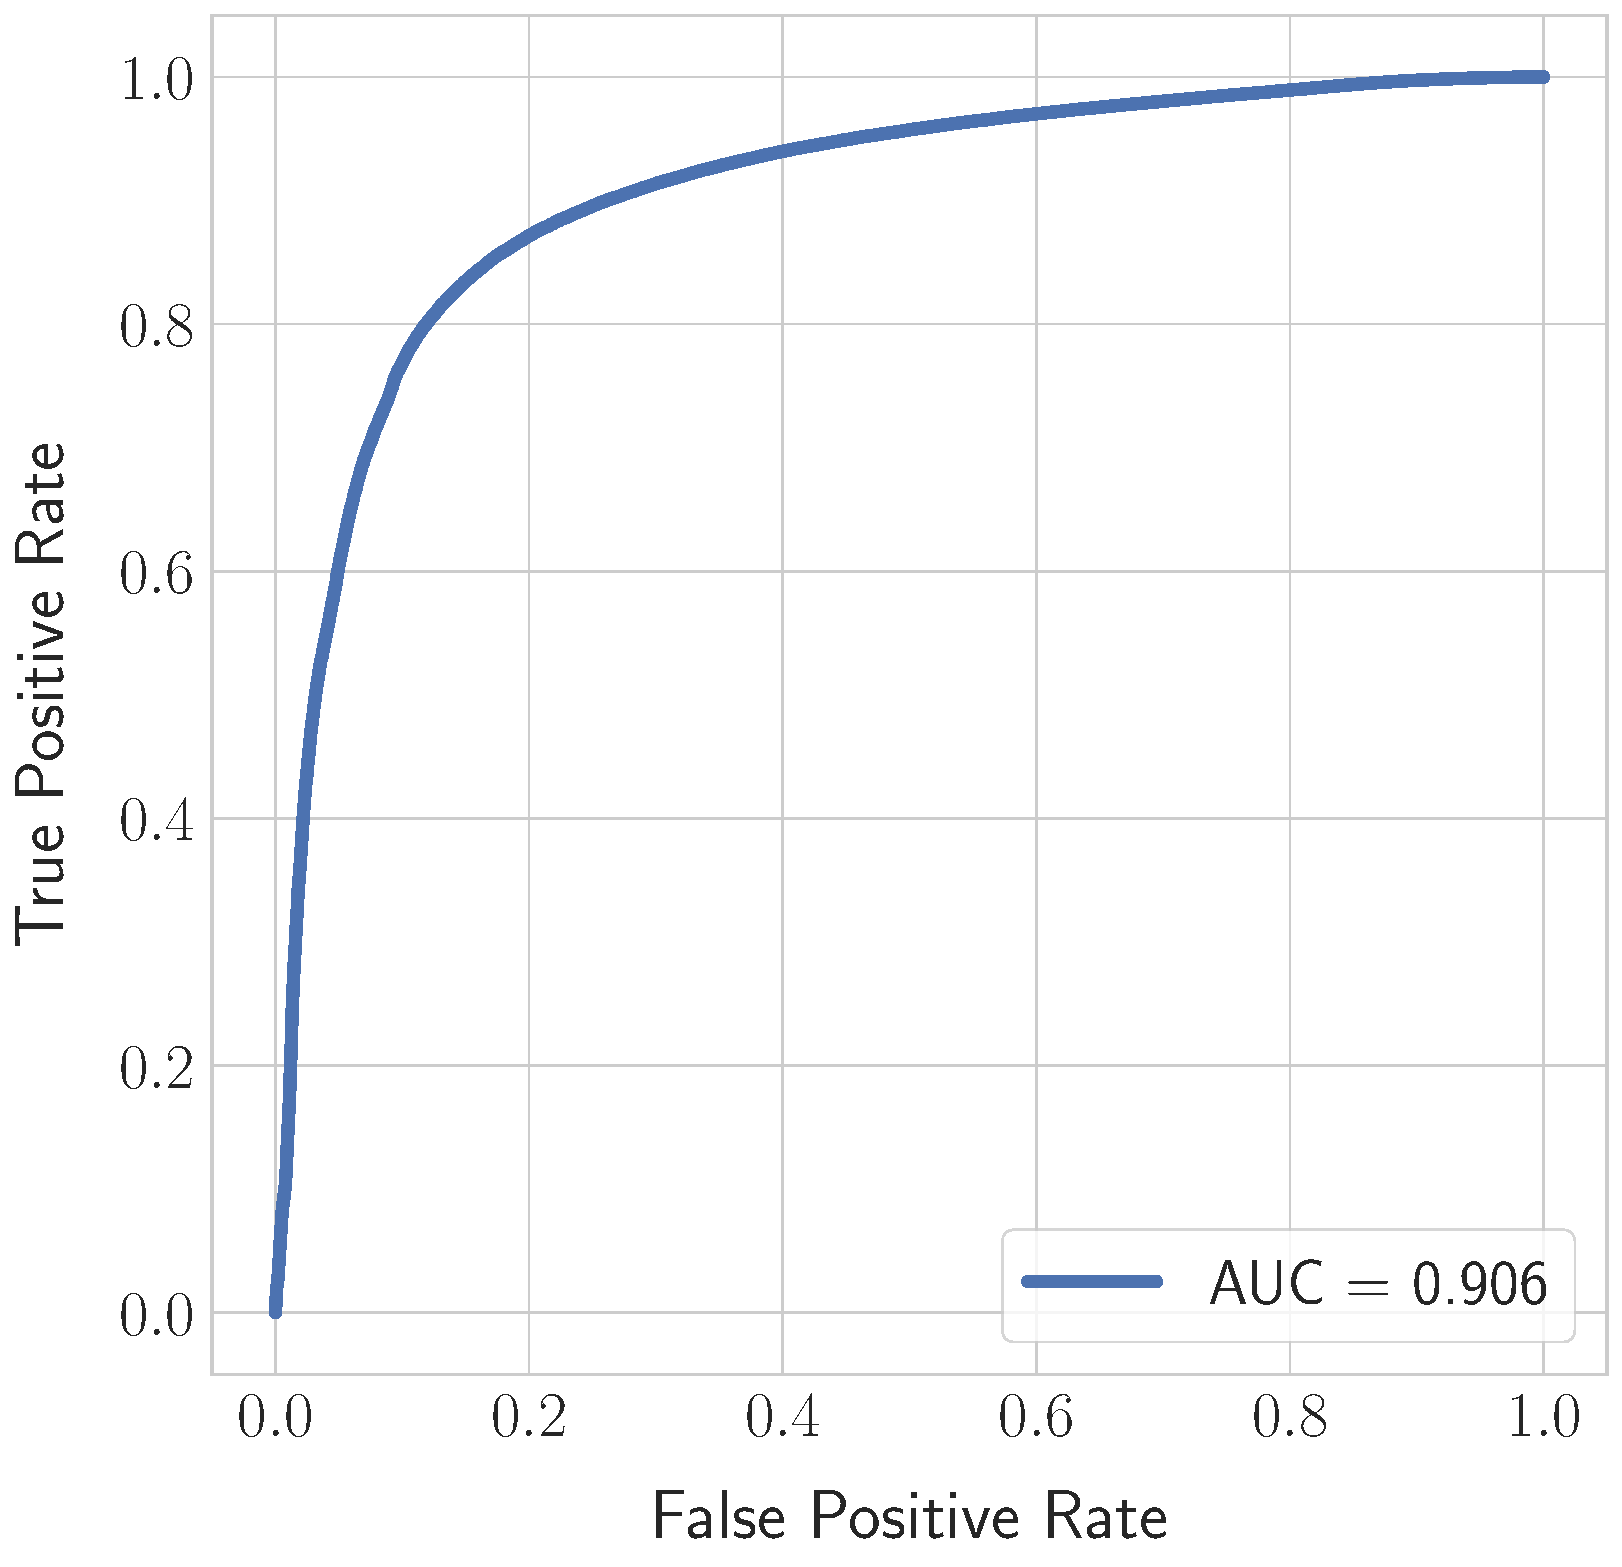
\includegraphics[width=0.6\textwidth]{Figures/roc_two_quark.pdf}
 	\caption{ ROC curve of SPA-NET applies on events with two reconstructable top quarks.}
 	\label{fig: roc two top}
 \end{figure}
\newpage
With regard to the more efficient performance of SPA-NET discussed in the last paragraph of Section \ref{sec:inv mass and reco eff}, our network achieved a lower AUC value in Figure \ref{fig: roc one top} and performs a remarkable ROC value in Figure \ref{fig: roc two top}.A possible solution we did not implement in this study is to train with the ``partial'' events by using the ``mask''\cite{Fenton:2020woz}\cite{Shmakov:2021qdz}.
\section{Reduction of computing time}\label{sec: reduce of time uasge}
The time required to compute SPA-NET is much lower than the $\chi^{2}$ method needs. We may compare the time they needed by considering the time complexity. The $\chi^{2}$ has a time complexity that scales approximately as $P(N,6)=\mathcal{O}(N^{6})$ where N is the number of jets in an event. The time complexity is $\chi^{2}$ proportional to the number of jets and this makes a limitation of maximum jets indeed. Considering a 2019 DELL XPS13 computer with Core i7-1065G7 1.30GHz CPU, the SPA-NET took an average of 4.4 ms for one event.  The $\chi^{2}$ took an average 20 ms in 6 jets events and 369 ms in $\ge$ 8 jets events. 
\section{Outlook}\label{sec:outlook}
Based on the design of SPA-NET, the input is a sequence of jet information and their relationships. The network considers the permutation relation between each subset and possible permutations. In case, a physics model which has a permutation relationship might be a good item to explore with SPA-NET. For example, $ttH$ all hadronic decay process or all hadronic four top decay process may be well-suited to study with SPA-NET. Furthermore, SPA-NET may have potential applications not only for the parton-jet assignment problem but for the clustering problem, graph matching problem, and so does another problem which contains a permutation symmetry. We plan to explore the SPA-NET with some interesting BSM problem, such as the tri-Higgs production in 2HDM model\cite{Low:2020iua}.



